\section{基于多重校验的时间隐通道鲁棒性方法设计}
\label{chap:hash:robustness}

本节主要对该时间隐通道构建方法中的鲁棒性方法,进行展开介绍,分别为基于HASH的码字间校验方法、基于CRC的码字自校验方法,以及基于异或校验的映射矩阵校验方法。对各方法的介绍,分别由调制阶段及解调阶段两个方面进行展开。

\subsection{基于HASH的码字间校验方法}
\label{chap:hash:robustness:hash}

\insertFigure{
	\begin{figure}
		\centering
        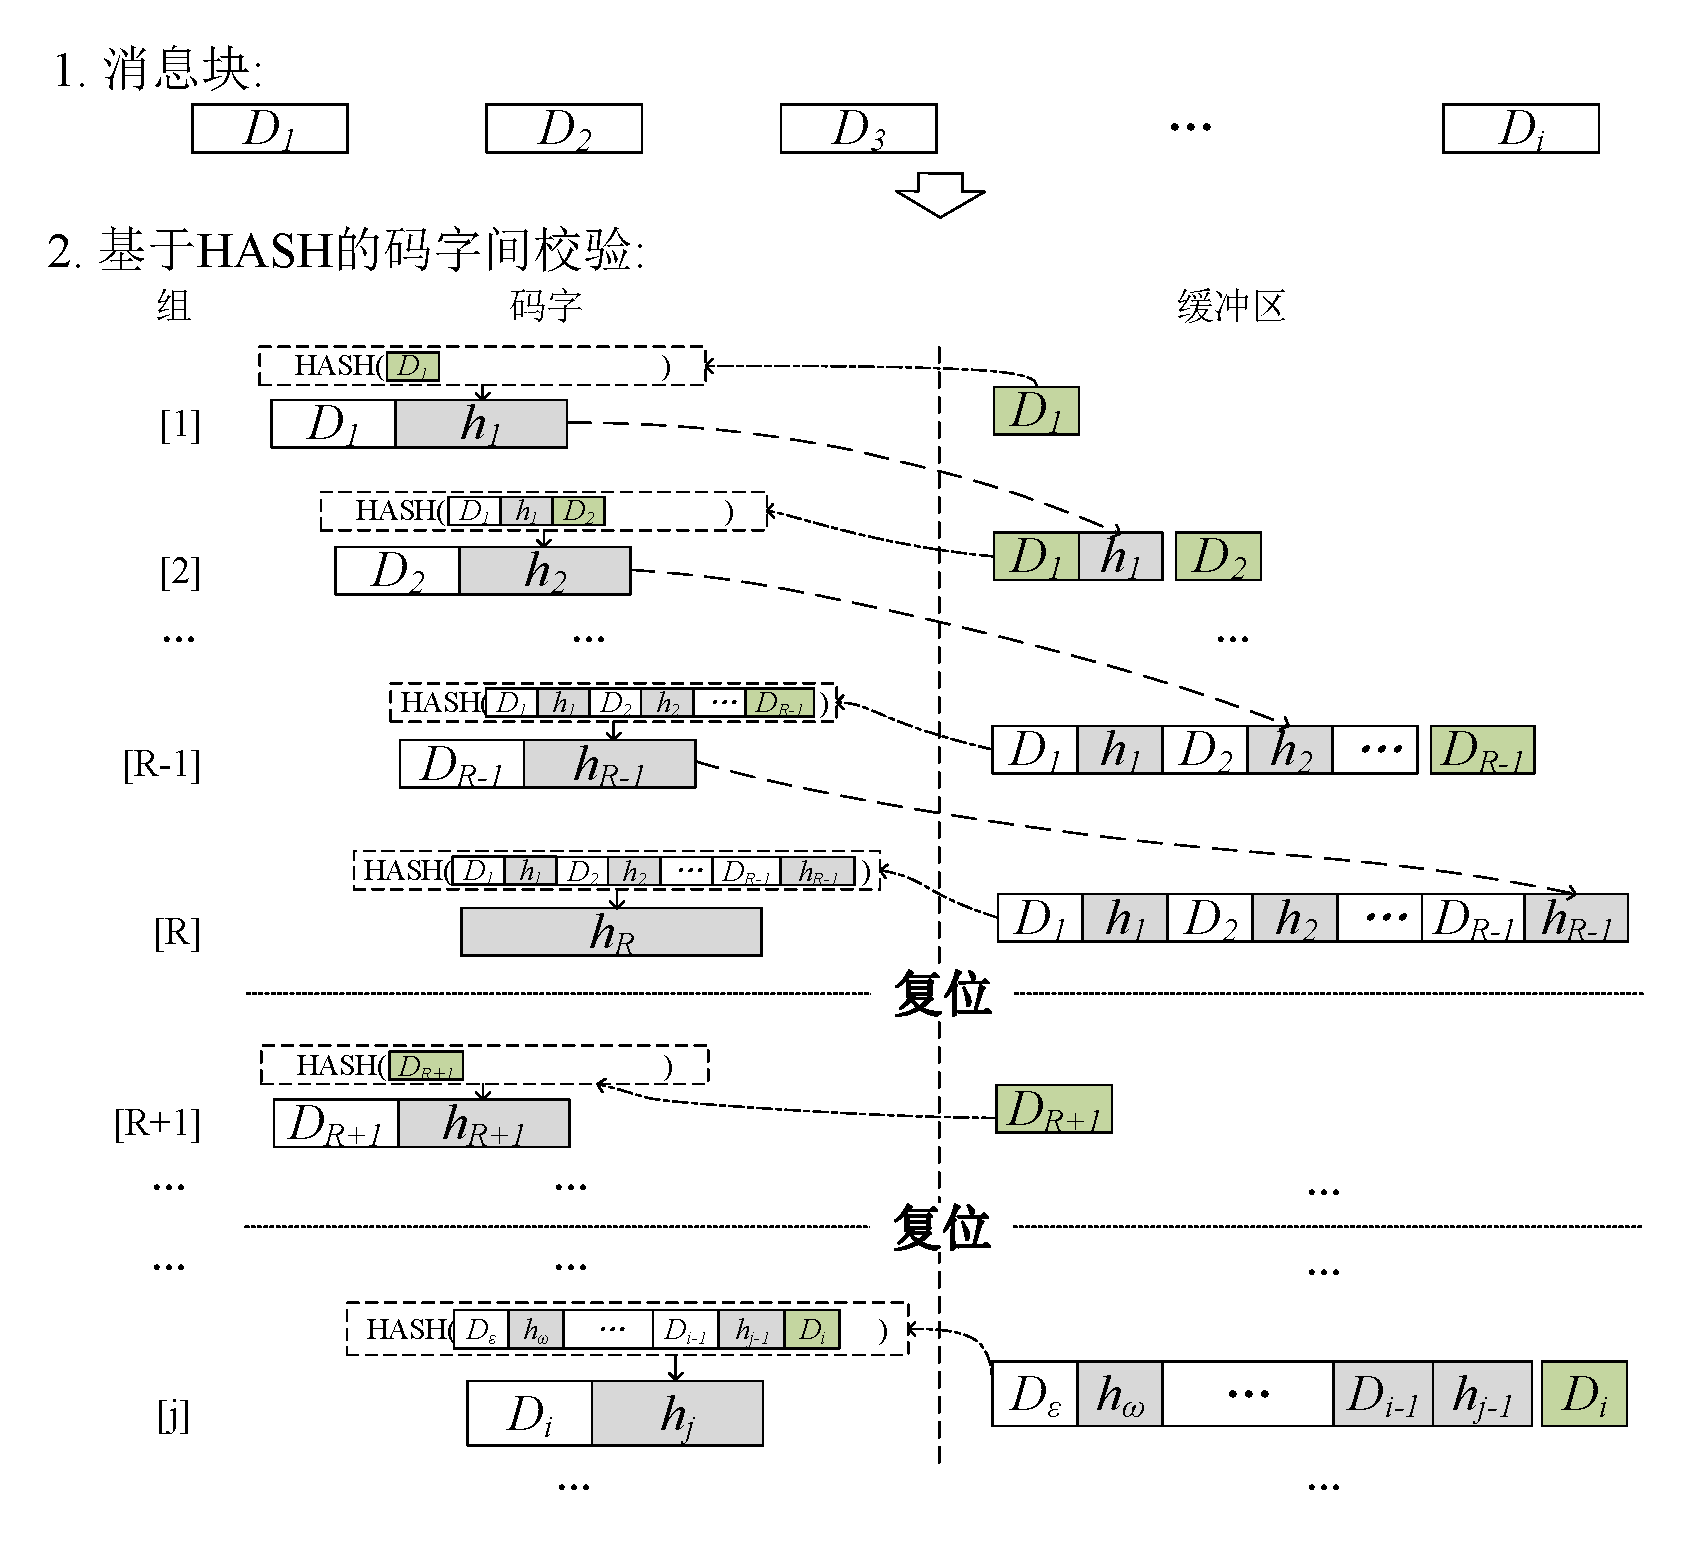
\includegraphics[width=0.9\textwidth]{chapters/chapter5/figures/hash-chain.pdf}
        \caption{基于HASH的码字间校验调制阶段示意图}
        \label{fig:5:hash-chain}
    \end{figure}
}
\insertEquation{
    \begin{equation}
        \label{equ:5:omega-j}
        \omega\ =\ {\left \lfloor{\frac{j\ -\ 1}{R}}\right \rfloor}\ \times\ {R\ +\ 1}
    \end{equation}
    \begin{equation}
        \label{euq:5:varepsilon-omega}
        \varepsilon\ =\ \omega\ -\ {\left \lfloor{\frac{\omega}{R}}\right \rfloor}
    \end{equation}
    \begin{equation}
        \label{euq:5:i-j}
        i\ =\ j\ -\ {\left \lfloor{\frac{j}{R}}\right \rfloor}
    \end{equation}
    \begin{equation}
        \label{euq:5:j-i}
        j\ =\ \left \lfloor{\frac{i}{R\ -\ 1}} \right \rfloor\ \times\ R\ +\ (i\ -\ 1)\ \%\ R\ +\ 1
    \end{equation}
}

基于HASH的码字间校验方法,涉及到的参数为$L_{HASH}$及$R$,以及用户的私有$Salt$及RTP中导出的随机$Seed$。通过计算多组码字之间的校验关系,建立码字间的关联关系。

\subsubsection{调制阶段}
\label{chap:hash:robustness:hash:modulation}

调制阶段,基于HASH的码字间校验如图\nref{fig:5:hash-chain}。建立码字间的校验关系,需要维持一个缓冲区,用于记录当前需要校验的数据信息。起始阶段缓冲区中为空,将第一组的数据块$D_{1}$添加到缓冲区中,并计算HASH$(D_{i})$作为$h_{1}$拼接到$D_{1}$末尾,同时将$h_{1}$添加到缓冲器。按照组号递增的顺序,依次迭代校验过程,到达组号为$R$时,缓冲区中数据已经累计得足够长,执行复位操作。复位阶段,生成特殊的校验块$h_{R}$,其长度为$BL+L_{HASH}$,并将缓冲区中数据清空。

按照复位周期R,依次计算所有的码字间校验块$h_{j}$,直至消息处理完毕。由于在复位周期添加了额外的校验码字,$D_{i}$与$h_{j}$中$i$与$j$的对应关系如公式(\nref{euq:5:j-i})及公式(\nref{euq:5:i-j})。图\nref{fig:5:hash-chain}中,复位后的起始消息块$D_{\varepsilon}$与组号$j$的关系,如公式(\nref{euq:5:varepsilon-omega})及公式(\nref{equ:5:omega-j})。

\subsubsection{解调阶段}
\label{chap:hash:robustness:hash:demodulation}

\insertFigure{
    \begin{figure}
        \centering
        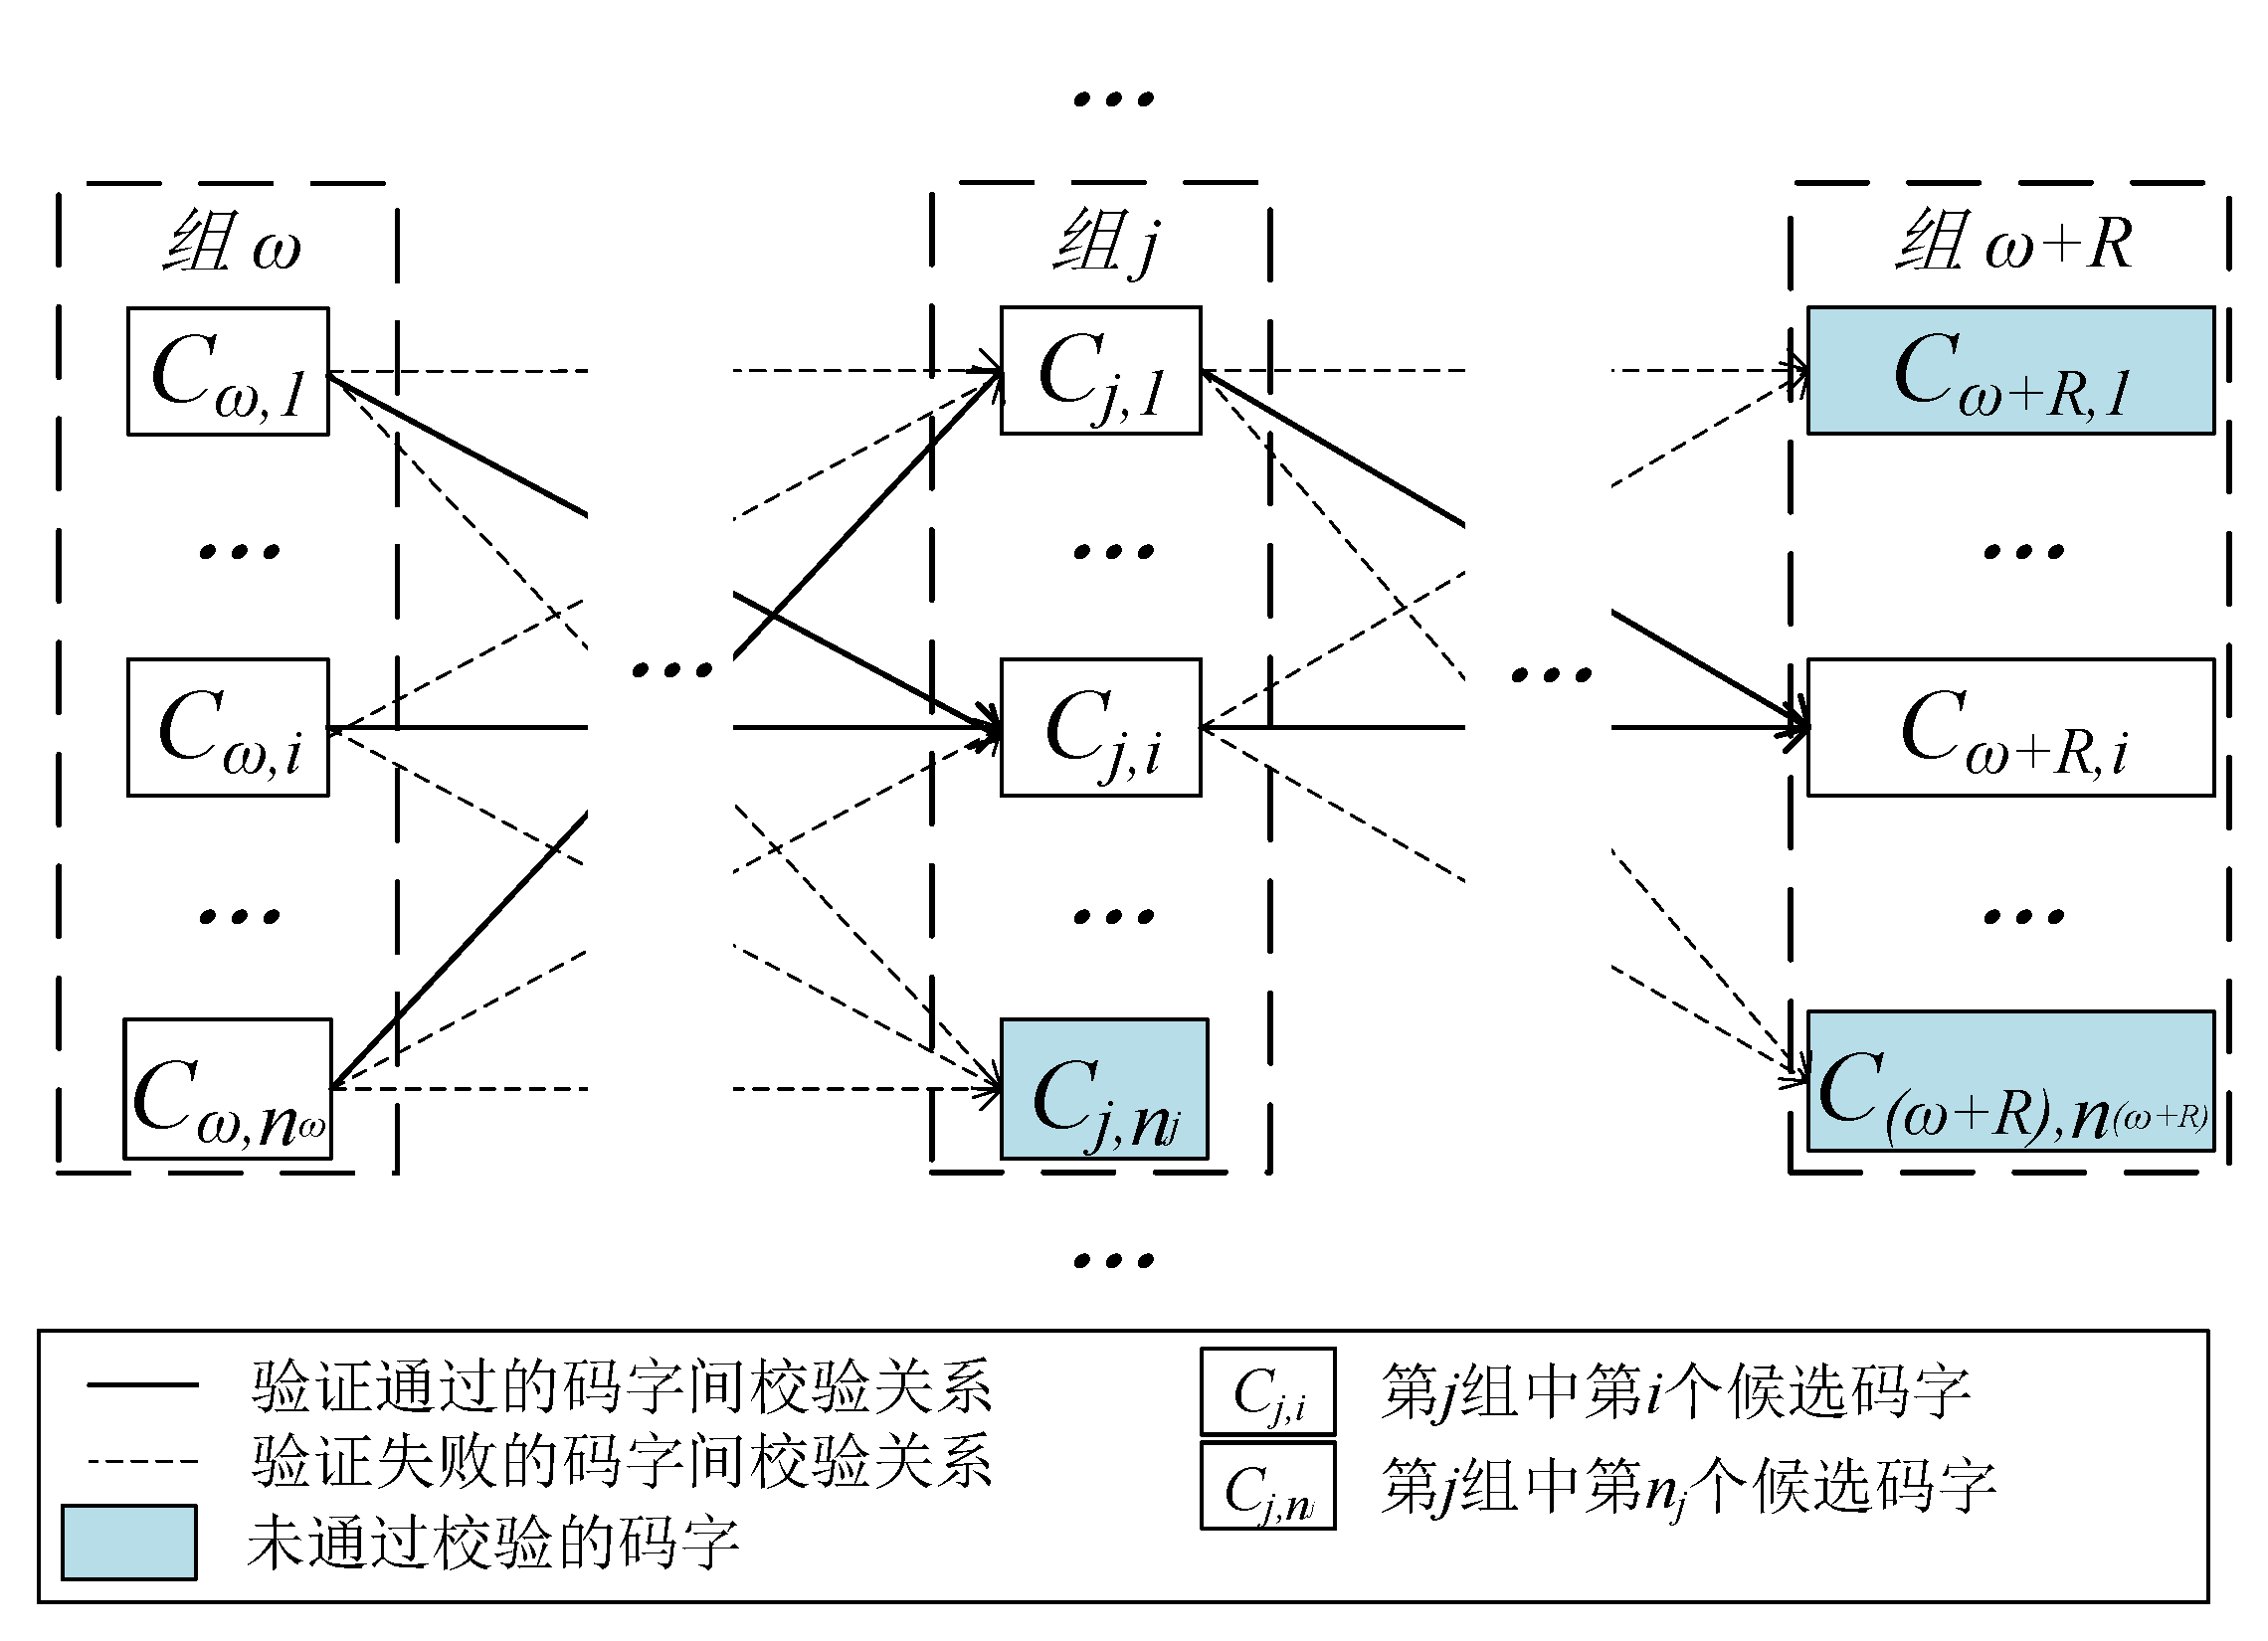
\includegraphics[width=0.8\textwidth]{chapters/chapter5/figures/hash-verification.pdf}
        \caption{基于HASH的码字间校验解调阶段示意图}
        \label{fig:5:hash-verification}
    \end{figure}
}

解调阶段,基于HASH的码字间校验如图\nref{fig:5:hash-verification},按照复位周期R进行切分,每个周期内的验证过程单独进行,在减小问题规模的同时防止噪声传播。对于每个周期内的候选码字集合$\{\{C_{1}',\cdots\}, \{C_{2}',\cdots \}, \cdots , \{C_{R}',\cdots\}\}$,所有的可行解构成了一个有向无环图,图的起点为$\{C_{1}',\cdots \}$,图中的每条边对应了一种码字间的关联关系。

解调过程与图遍历过程类似,由起点开始,对所有的边进行验证,只有符合基于HASH的码字校验时,才保留,否则将边由图中删除。对于非$R$组的节点,当节点出度为0时,意味着没有满足要求的后继节点,判断该节点为网络噪声,在图中将该节点移除。最终,当有一条有起点出发的路径达到第R组的节点,即为一种可能的码字组合,如图\nref{fig:5:demodulation-flow}码字间校验。在网络噪声的干扰下,最终可能存在多种候选组合,根据图中节点入度与出度的意义,选择路径中各节点入度之和最大的路径,作为最终结果。

\subsection{基于CRC的码字自校验方法}
\label{chap:hash:robustness:crc}

\insertContents{
    \begin{algorithm}[t]
        \renewcommand{\algorithmcfname}{算法}
        \caption{码字生成}
        \label{alg:5:codeword-generation}
        \LinesNumbered
        \KwIn{$message$,\ $BL$,\ $L_{HASH}$,\ $L_{CRC}$,\ $R$,\ $Salt$,\ $Seed$}
        \KwOut{$C\ \leftarrow\ \{\}$}
        $D\ \leftarrow$\ group into blocks$(message,\ BL)$ \\
        $modulated\_sections\ \leftarrow\ NULL$ \\
        $salt\ \leftarrow\ Salt\ \oplus\ Seed$ \\
        \For {$D_i$\ in\ $D$} {
            $j\ \leftarrow\ \left \lfloor{\frac{i}{R\ -\ 1}} \right \rfloor\ \times\ R\ +\ (i\ -\ 1)\ \%\ R\ +\ 1$ \\
            append\ $D_i$\ to\ $modulated\_sections$ \\
            $h_j\ \leftarrow\ L_{HASH}$\ bits\ of\ HASH\ ($salt\ //\ modulated\_sections\ //\ salt$) \\
            $C_j\ \leftarrow$\ append\ $h_j$\ to\ $D_i$ \\
            append\ $h_j$\ to\ $modulated\_sections$ \\
            append\ $C_j$\ to\ $C$ \\
            \If {$i$\ mod\ $R$\ ==\ 0} {
                $C_{j\ +\ 1}\ \leftarrow\ (L_{Codeword} - L_{CRC})$\ bits of HASH\ ($salt\ //\ modulated\_sections\ //\ salt$) \\
                append\ $C_{j\ +\ 1}$\ to\ $C$ \\
                $modulated\_sections\ \leftarrow\ NULL$ \\
            }
        }
        \For {$C_j$ in $C$} {
            $C_j\ \leftarrow$\ append\ $L_{CRC}$\ bits of CRC32\ ($salt\ //\ C_j\ //\ salt$)\ to\ $C_j$
        }
        \Return $C$
    \end{algorithm}
}


基于CRC的码字自校验方法,通过在码字$C_{j}$中设置CRC校验块$v_{j}$,验证$D_{i}//h_{j}$部分的正确性。给校验方法针对单个码字,没有码字间的依赖关系,因此调制及解调过程效率较高。

\subsubsection{调制阶段}
\label{chap:hash:robustness:crc:modulation}

\insertFigure{
	\begin{figure}
		\centering
        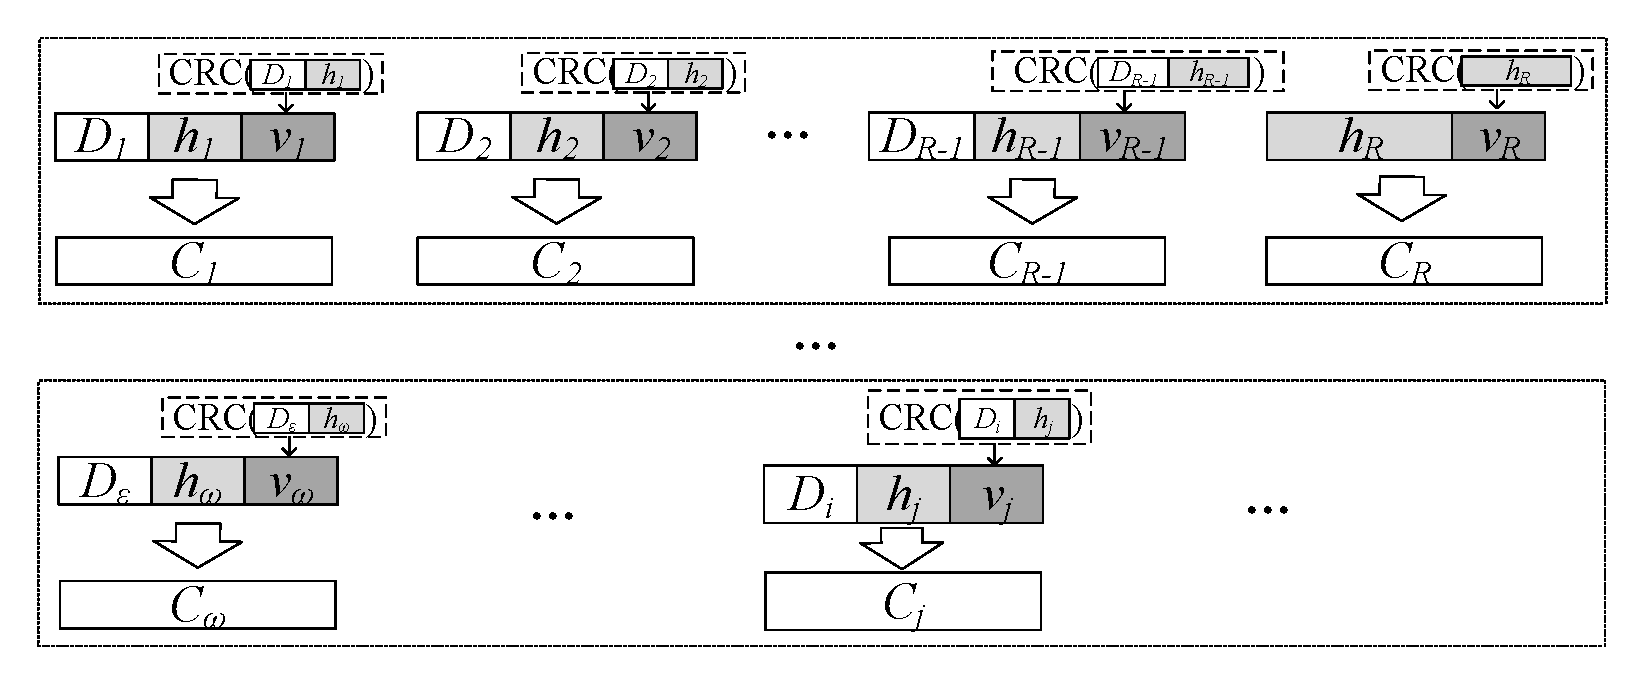
\includegraphics[width=0.8\textwidth]{chapters/chapter5/figures/crc-generation.pdf}
        \caption{基于CRC的码字自校验调制阶段示意图}
        \label{fig:5:crc-generation}
    \end{figure}
}

调制阶段,基于CRC的码字间自校验如图\nref{fig:5:crc-generation}。码字由$D_{i}$、$h_{j}$及$v_{j}$三部分组成,基于CRC的码字校验块即$v_{j}$,根据传输参数$L_{CRC}$设定,$v_{j}$为CRC散列结果中的部分值。

基于CRC的码字自校验计算完毕后,码字的各组成部分均准备完毕,组合即可得到码字$C_{j}$。算法\nref{alg:5:codeword-generation}描述了由隐蔽消息到码字的处理过程,包含消息分组及码字生成两个部分,其中码字生成包含了计算基于HASH的码字间校验信息,以及计算基于CRC的码字自校验信息两种校验方式。在计算HASH摘要及CRC散列值中,均进行加盐操作,保证校验信息的随机性。

\subsubsection{解调阶段}
\label{chap:hash:robustness:crc:demodulation}

\insertContents{
    \begin{algorithm}[t]
        \renewcommand{\algorithmcfname}{算法}
        \caption{有效码字鉴别}
        \label{alg:5:codeword-identification}
        \LinesNumbered
        \KwIn{$S'$,\ $L_{CRC}$,\ $Salt$,\ $Seed$}
        \KwOut{$C'\ \leftarrow\ \{\}$}
        $salt\ \leftarrow\ Salt\ \oplus\ Seed$ \\
        \For {\{${S_j'}$\}\ in\ $S'$} {
            $\{C_j'\}\ \leftarrow\ \{\}$ \\
            \For {$S_j'$\ in\ \{$S_j'$\}} {
                $v_j',\ h_j',\ D_j'\ \leftarrow$\ extracted from $S_j'$ \\
                $crc32\_result\ \leftarrow\ L_{CRC}$ bits of CRC32\ ($salt\ //\ D_j'\ //\ h_j'\ //\ salt$) \\
                \If {$v_j'$ == $crc32\_result$} {
                    append\ $S_j'$\ to\ \{$C_j'$\}
                }
            }
            append\ \{$C_j'$\}\ to\ $C'$
        }
        \Return $C'$
    \end{algorithm}
}


解调阶段的算法描述如算法\nref{alg:5:codeword-identification},对于候选符号,只有其对应的码字符合校验规则,符号-码字转换结果才是有效的,否则噪声会被引入到基于HASH的码字间检验过程。解调过程种需要重新计算CRC校验部分,处理流程与调制时完全一致,并且保证加盐信息一致,才可以完成校验。

\subsection{基于异或的映射矩阵校验方法}
\label{chap:hash:robustness:xor}

\insertFigure{
	\begin{figure}
		\centering
        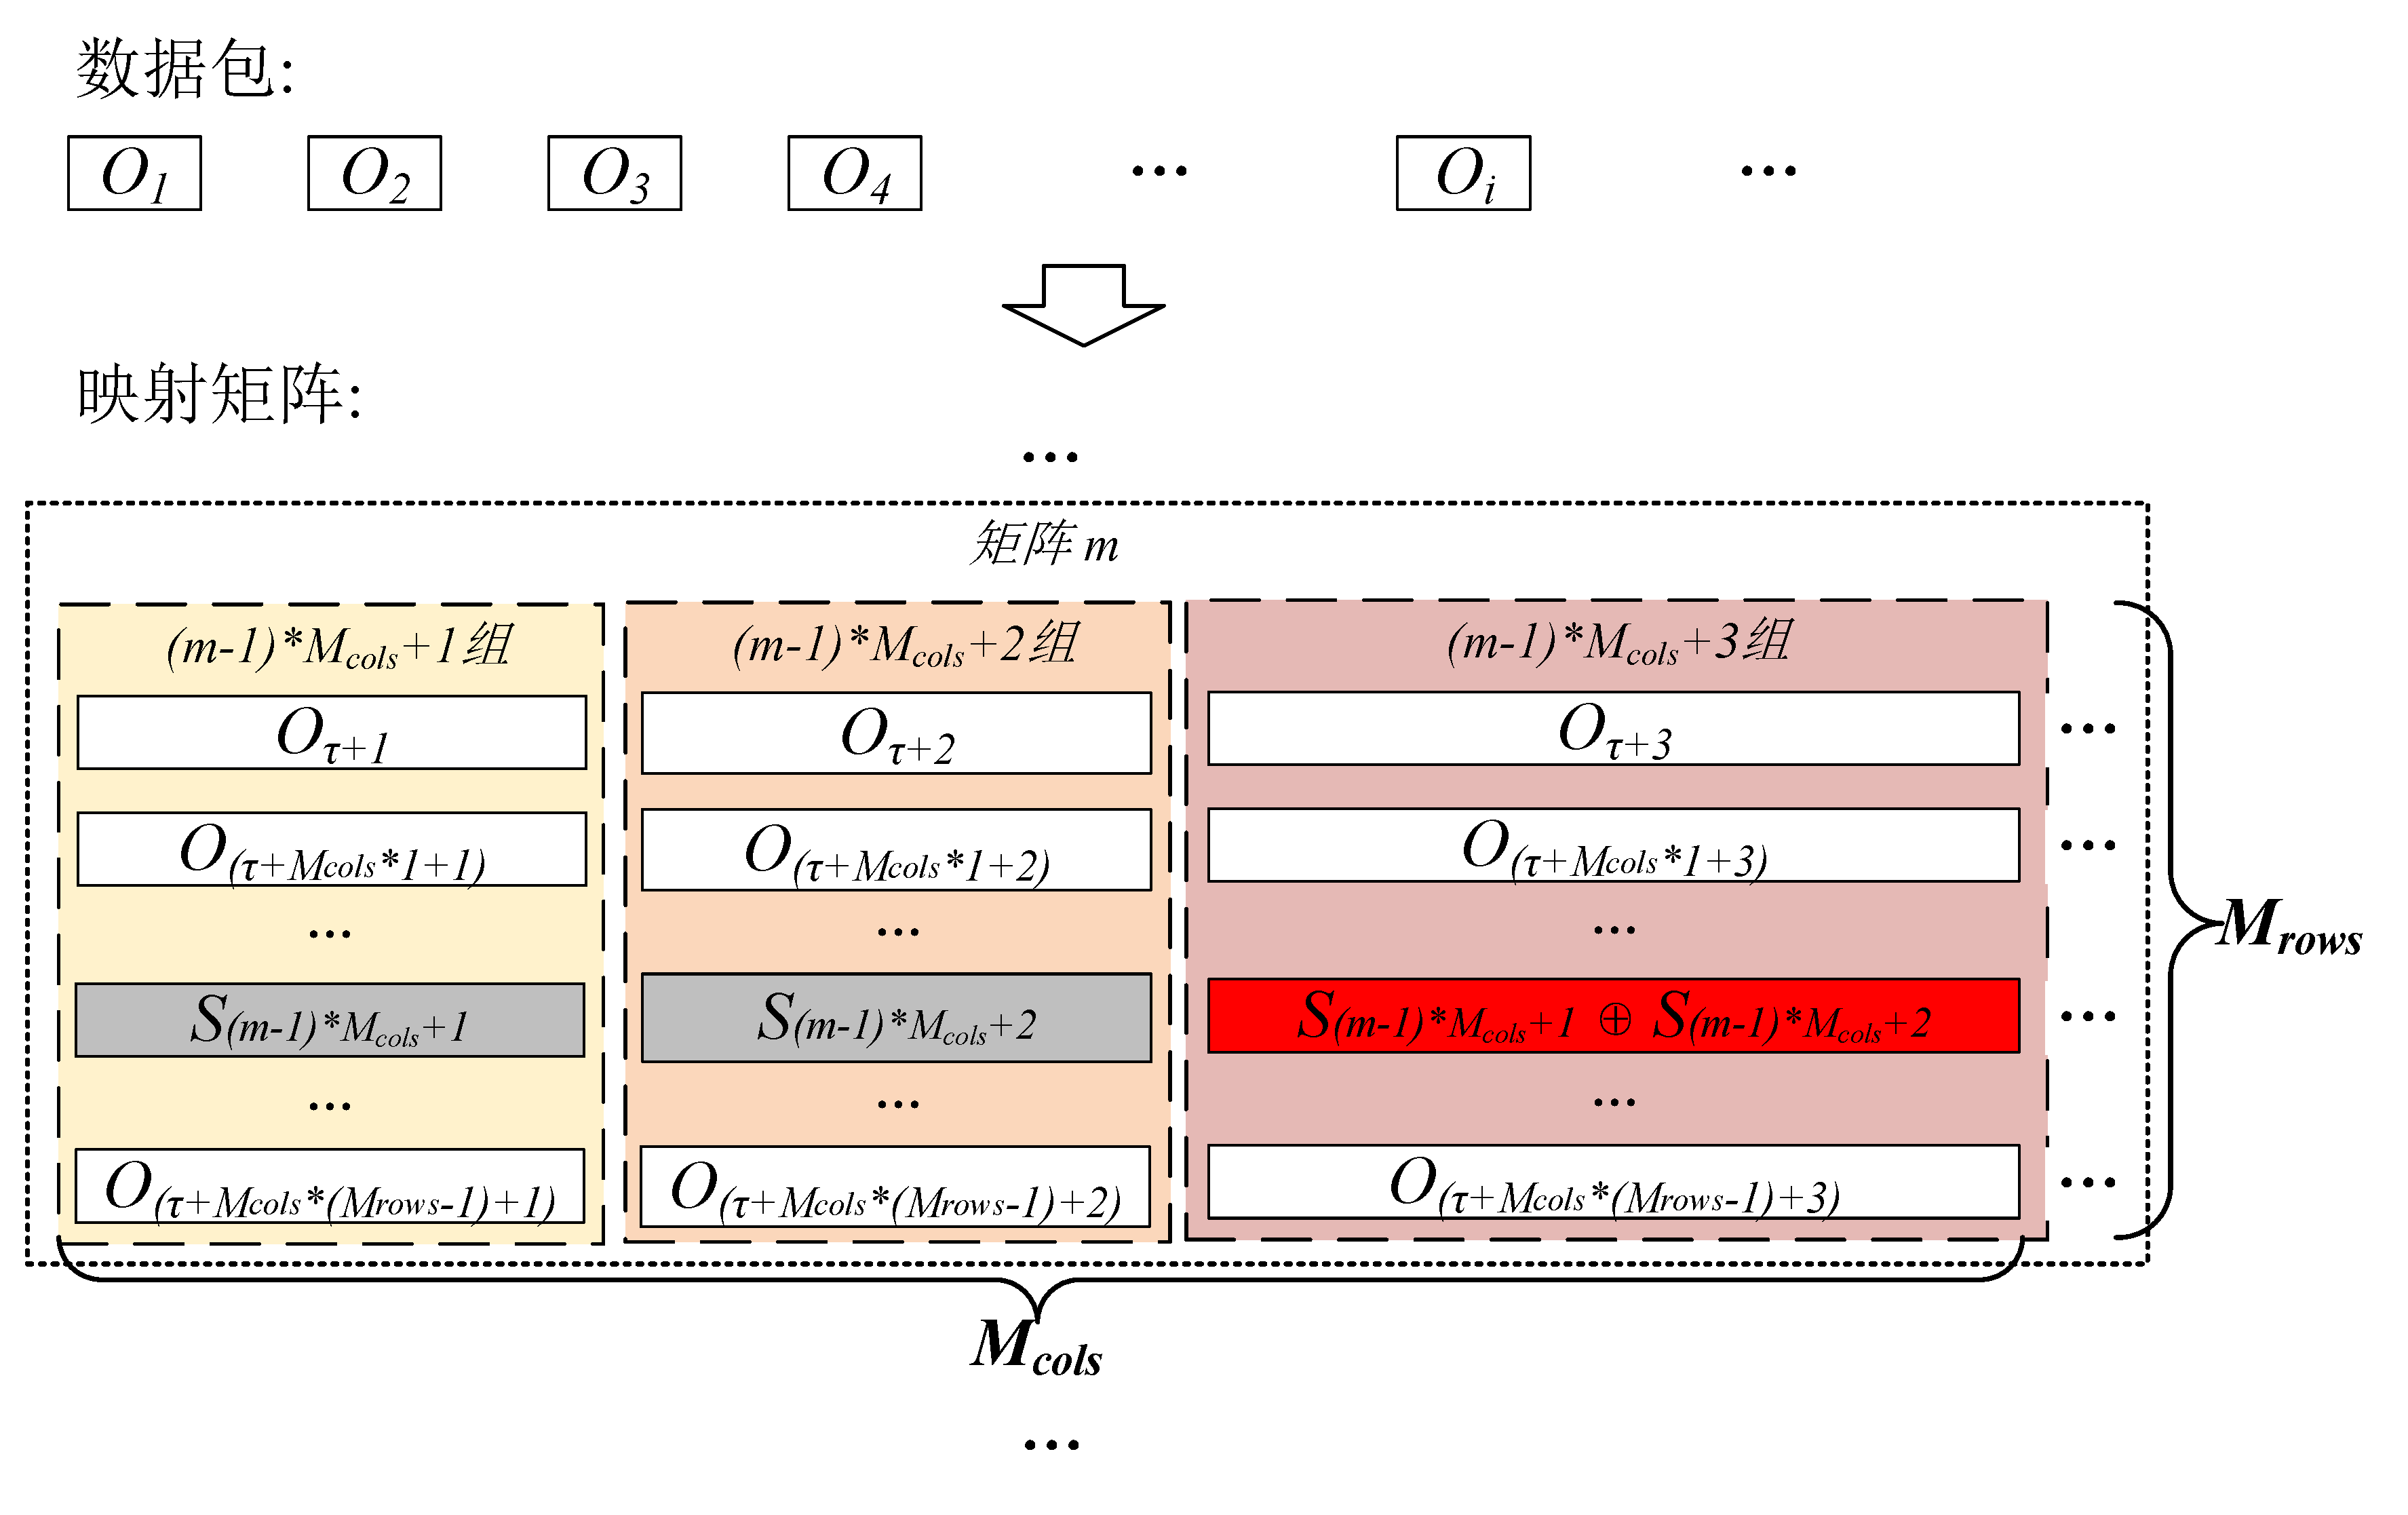
\includegraphics[width=0.95\textwidth]{chapters/chapter5/figures/mapping-matrix.pdf}
        \caption{映射矩阵及异或校验示意图}
        \label{fig:5:mapping-matrix}
    \end{figure}
}

映射矩阵实现了由码字到数据包序号的转换,并在矩阵内部添加了基于异或校验的符号校验,同时矩阵的列数为可调整的参数,有利于降低连续丢包噪声的干扰。

\subsubsection{调制阶段}
\label{chap:hash:robustness:xor:modulation}

映射矩阵及矩阵中的异或校验如图\nref{fig:5:mapping-matrix},数据包序号按照行序进行填充,对于第$m$个映射矩阵,矩阵由$O_{\tau +1}$开始,其中$\tau$由公式(\nref{equ:5:tau})定义。矩阵的行数$M_{rows}$与符号的表示范围有关,而符号由码字转换得到,因此$M_{rows}$由公式(\nref{equ:5:m-rows})根据$L_{Codeword}$计算得出。

\insertEquation{
    \begin{equation}
        \label{equ:5:m-rows}
        M_{rows}\ =\ 2^{L_{Codeword}}
    \end{equation}
    \begin{equation}
        \label{equ:5:tau}
        \tau\ =\ M_{cols}\ \times\ (m\ -\ 1)\ \times\ M_{rows}
    \end{equation}
    \begin{equation}
        \label{equ:5:p_k}
        P_k\ (k,\ S_k)\ =\ \left \lfloor{\frac{k\ -\ 1}{M_{cols}}}\right \rfloor \times (M_{rows} \times M_{cols})\ +\ M_{cols} \times (S_k\ -\ 1)\ +\ (k\ -\ 1)\ \%\ M_{cols}\ +\ 1
    \end{equation}
}
\insertContents{
    \begin{algorithm}[t]
        \renewcommand{\algorithmcfname}{算法}
        \caption{码字转换为序号}
        \label{alg:5:codeword-to-sequence}
        \LinesNumbered
        \KwIn{$C$,\ $L_{Codeword}$,\ $M_{cols}$,\ $Salt$,\ $Seed$}
        \KwOut{$P\ \leftarrow\ \{\}$}
        $S\ \leftarrow\ \{\}$ \\
        $offset\ \leftarrow$\ Random\ ($Salt \oplus Seed$) \\
        \For {$C_j$ in $C$} {
            $S_k\ \leftarrow$\ Integer\ ($C_j$)\ +\ 1 \\
            append\ $S_k$\ to\ $S$ \\
            \If {$j$\ mod\ 2\ ==\ 0} {
                append\ $S_k\oplus S_{k-1}$\ to $S$
            }
        }
        \For {$S_k$\ in\ $S$} {
            $offset\ \leftarrow$\ Random\ ($offset$) \\
            $S_k\ \leftarrow\ (S_k\ +\ offset)\ mod\ (2^{L_{Codeword}})\ +\ 1$
        }
        \For {$S_k$\ in\ $S$} {
            $P_k\ \leftarrow\ P_k\ (k,\ S_k)$ \\
            append\ $P_k$\ to\ $P$
        }
        \Return $P$
    \end{algorithm}
}

映射矩阵中,每一个数据包序号均有其坐标值,纵坐标代表符号,也就是相对丢包位置;横坐标表示在矩阵中的相对分组序号,矩阵中的每一列构成一个符号传输组。映射矩阵中,基于异或校验的校验符号,插入在每两个数据符号之后,如图\nref{fig:5:mapping-matrix}中,第$(m-1)\times M_{cols}+3$组需要添加异或校验符号,则插入前两组符号的异或值$S_{(m-1)\times M_{cols}+1}\oplus S_{(m-1)\times M_{cols}+2}$。异或校验模式,生成的符号3个为一组,要求$M_{cols}\%3=0$,从而一个映射矩阵刚好满足对所有符号的校验。

码字到数据包序号的转换过程,如算法\nref{alg:5:codeword-to-sequence},输入的参数包括码字集合、传输参数及随机数种子。在开始处理前,首先根据$Salt$及$Seed$生成随机数种子,用于生成每组符号的偏移量。转换过程主要包含三个部分,第一个部分是添加异或校验,第二个部分是添加随机偏移量,第三个部分是符号转换为序号,三部分各对应一个循环遍历过程。

在第一部分添加异或校验时,先将二进制码字转换为十进制,并添加到符号集合$S$。按照每两组符号添加一组异或校验的模式,判断当进行到偶数组时,将前两组符号进行异或,然后加入到符号集合$S$。第二部分添加随机偏移量,每次都会迭代伪随机数发生器,从而即使是相同的符号,处理后的结果也不会完全相同。第三部分将符号映射到数据序号,每个符号及其组号,构成一个$[k,\ S_{k}]$二元组,对应着矩阵中的位置,按照公式(\nref{equ:5:p_k}),转换为全局的数据包序号,该阶段处理完毕。

\subsubsection{解调阶段}
\label{chap:hash:robustness:xor:demodulation}

\insertEquation{
    \begin{equation}
    \label{equ:5:get-k}
        k\ =\ \left \lfloor{\frac{P'}{M_{rows}\ \times\ M_{cols}}}\right \rfloor\ \times\ M_{cols}\ +\ (P'\ -\ 1)\ \%\ M_{cols}\ +\ 1
    \end{equation}
    \begin{equation}
    \label{equ:5:get-s}
        S_j'\ =\ \left \lfloor{\frac{P_j'\ -\ M_{rows}\ \times\ M_{cols}\ \times\ \left \lfloor{\frac{P_j'}{M_{rows}\ \times\ M_{cols}}}\right \rfloor\ -\ 1}{M_{cols}}}\right \rfloor
    \end{equation}
    \begin{equation}
    \label{equ:5:remove-offset}
        S_j'\ =\ ({S_j'\ -\ offset\%({2^{L_{Codeword}}})\ +\ 2^{L_{Codeword}}})\ \%\ (2^{L_{Codeword}})\ +\ 1
    \end{equation}
}

解调过程中,通过映射矩阵提取每组的符号信息,同时对插入的异或校验符号进行验证。接收方通过监听传输过程,获取丢包序号$P'$,要得到消息内容,需要解析该序号对应的符号以及匹配的组号。组号的计算如公式(\nref{equ:5:get-k}),在一次传输过程中,映射矩阵的规模是确定的,通过判断丢包位置对应的矩阵位置,结合矩阵中的偏移信息,即可解析出组号$k$。

符号的解析方式,如公式(\nref{equ:5:get-s}),由于符号是相对的偏移位置,因此只需要定位到映射矩阵内部即可。受噪声影响,每一组中的符号可能有多个,因此得到的结果为$\{\{S_1',\cdots\},\{S_2',\cdots\},\cdots, \{S_k',\cdots\}, \cdots\}$。

按照调制过程中的处理顺序,符号首先需要消除随机偏移量,才可以进行进一步的鉴别工作,该操作过程如公式(\nref{equ:5:remove-offset})。其中,每一组的$offset$与调制阶段采用相同的方式,迭代伪随机数发生器得到。

通过验证符号间的异或校验关系,即可完成多层校验的第一层校验,按照每三组符号一组的方式,校验所有的组合。校验过程中,利用异或关系的特征,符合规则的符号$S_1'$,$S_2'$,$S_3'$应当满足$S_1'\oplus S_2'\oplus S_3' = 0$,对于无法通过验证的符号,可以判断为噪声丢弃。